\section{Results and Discussion} \label{sec:results}

\begin{figure}

\begin{subfigure}[c]{\linewidth} \centering
\begin{minipage}[c]{0.08\linewidth} \flushright
    \caption{\rotatebox[origin=c]{90}{25 cycles}}
    \label{fig:tagged_25}
  \end{minipage}%
  \begin{minipage}[c]{0.92\linewidth}
    \includegraphics[width=\textwidth,height=0.6in,trim={0 0.81cm 0 0},clip]{binder-wse-sketches/binder/teeplots/genome=hsurftiltedsticky_tagged+replicate=e4ea2071-8228-42de-af8c-879cedff9ba7+viz=draw-biopython-tree+ext=}
  \end{minipage}%
\end{subfigure}

\vspace{-1ex}

\begin{subfigure}[c]{\linewidth} \centering
\begin{minipage}[c]{0.08\linewidth} \flushright
    \caption{\rotatebox[origin=c]{90}{50 cycles}}
    \label{fig:tagged_50}
  \end{minipage}%
  \begin{minipage}[c]{0.92\linewidth}
    \includegraphics[width=\textwidth,height=0.6in,trim={0 0.81cm 0 0},clip]{binder-wse-sketches/binder/teeplots/genome=hsurftiltedsticky_tagged+replicate=3d55af5f-7714-45da-9276-e860f46b4d94+viz=draw-biopython-tree+ext=}
  \end{minipage}%
\end{subfigure}

\vspace{-1ex}

\begin{subfigure}[c]{\linewidth} \centering
  \begin{minipage}[c]{0.08\linewidth} \flushright
    \caption{\rotatebox[origin=c]{90}{100 cycles}}
    \label{fig:tagged_100}
  \end{minipage}%
  \begin{minipage}[c]{0.92\linewidth}
    \includegraphics[width=\textwidth,height=0.6in,trim={0 0.81cm 0 0},clip]{binder-wse-sketches/binder/teeplots/genome=hsurftiltedsticky_tagged+replicate=932aa302-becb-47e8-9712-7f550b02364c+viz=draw-biopython-tree+ext=}
  \end{minipage}%
\end{subfigure}

\vspace{-1ex}

\begin{subfigure}[c]{\linewidth} \centering
  \begin{minipage}[c]{0.08\linewidth} \flushright
    \caption{\rotatebox[origin=c]{90}{250 cycles}}
    \label{fig:tagged_250}
  \end{minipage}%
  \begin{minipage}[c]{0.92\linewidth}
    \includegraphics[width=\textwidth,height=0.8in]{binder-wse-sketches/binder/teeplots/genome=hsurftiltedsticky_tagged+replicate=42dbcbb3-b803-41a4-9285-4a450bfad6ed+viz=draw-biopython-tree+ext=}
  \end{minipage}%
\end{subfigure}

\caption{%
\textbf{Clade Validation Trial.}
\footnotesize
Example phylogenies reconstructed from runs of increasing duration on virtual grid of nine hardware-simulated PEs.
Founding genomes were tagged with random 16-byte identifier values, which were held constant over the course of simulation (Supplementary Figure \ref{fig:genome-layout}).
Color-coding indicates each sampled taxon's founding ancestor according to this identifier value.
Simulation performed under drift conditions.
}
\label{fig:tagged}

\end{figure}


\begin{figure*}
  \centering
  \includegraphics[width=\textwidth]{binder-reconstruction-quality/binder/surf-vs-col/outplots/surf-vs-col-table}
  \caption{%
    Column (red) vs. surface (blue) performance.
    For heatmap charts, +'s indicate small, medium, and large effect sizes using the Cliff's delta statistic and *'s indicate statistical significance at $\alpha = 0.05$ via Mann-Whitney U test.
  }
  \label{fig:col-vs-surf}
\end{figure*}


\subsection{Surface Algorithm Benchmark}

\begin{figure*}
  \centering
  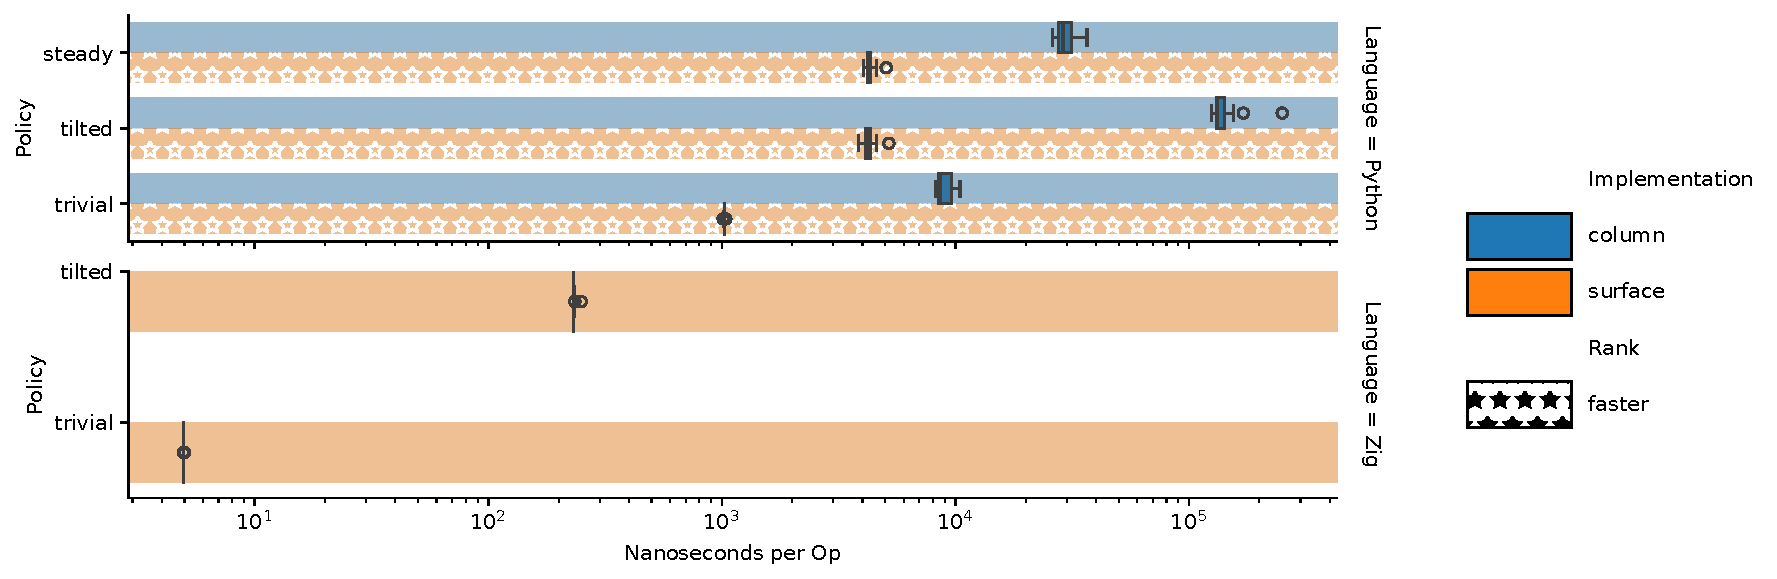
\includegraphics[width=0.85\textwidth,trim={0 0 0 0.4in
  }, clip]{binder-wafer-scale/binder/teeplots/all=false+hue=implementation+orient=h+row=language+score=nanoseconds-per-op+viz=peckplot+x=nanoseconds-per-op+y=policy+y-group=outer+ext=}

\vspace{-2.5ex}

  \caption{%
    \textbf{Hereditary stratigraphy algorithm benchmarks.}
    \footnotesize
    Comparison of per-generation operation time for column- and surface-based steady and tilted retention policies, lower is better.
  Top and bottom panels show Python and Zig implementations, respectively.
    Trivial is a simple harcoded retention decision, provided as a baseline control.
    Background hatching indicates significant outcome (Mann-Whitney U test; $n=20$).
  }
  \label{fig:benchmarking}
  \vspace{-0.2in}
\end{figure*}


We performed benchmarking experiments to assess the computational performance of our new surface-based algorithms.
Due to limited completed implementations of compiled-language algorithms, we performed the bulk of benchmarking using the Python implementations.
While Python is an interpreted language and the Python-implemented algorithms weren't specifically implemented to maximize performance, and has an intrinsic performance penalty due to that, the algorithms were all in the same footing and we use the ``optimize''' flag to strip assert statements out of the benchmarks.
However, in the process of porting the tilted surface algorithm over to Cerebras Software Language we did create an implementation of that algorithm in Zig which is a compiled language and is capable of compiler optimizations.
We augment the Python with a benchmark of this algorithm.
Figure \ref{fig:benchmarking} provides an overview of results.

% https://github.com/mmore500/hstrat-surface-concept/blob/51d636d768d474fc5148b9fcaa199c1b7776e915/benchmark.ipynb
We found that the Python implementations of the surface tilted and steady algorithms both took around 4,200ns per operation (SEM c. 50; $n=20$).
For context, this was about $4\times$ the measured time for a surface placement using a trivial calculation (SEM c. 0.05; $n=20$).
The column implementations of steady and tilted fared much worse, taking about $7\times$ and $34\times$ the execution time per operation compared to the surface operations.
Mann-Whitney U tests confirmed that surface implemnetations significantly outperformed their column counterparts. (Figure \ref{fig:benchmarking}).

% https://github.com/mmore500/wse-sketches/blob/d4ab0155f63ff5809f8eeca1169ad9b272c30a68/binder/benchmark.ipynb
Zig implementation of tilted surface:
233 ns per operation (SEM 0.9; $n=20$).
This was $47\times$ the measured time for a trivial placement calculation (SEM 0.2; $n=20$).
For context, this time a little more than twice the amount of time required for a main memory access in contemporary computing hardware \citep{markus2022memory}.
